\chapter{Sensor Payload}
The sensor payload is composed by 3 subsystems:
\begin{enumerate}
    \item Raspberry Pi 3b+
    \item Analogue Front End (AFE) by Alphasense equipped with 3 gas sensors (NO, NO2 and CO) and a PID (VOCs) sensor
    \item Nova SDS011 particulate sensor board for PM2.5 and PM10
\end{enumerate}
A student bachelor thesis performed a FEM study on the sensors and the Pi3b+ support platforms. The
elements have been studied in order to present a high resistance to vibrations and to allow the sensors
and the boards to be housed in the most safest way. In addition, the study also sought to design very
light components: the boards were built with a 3D PLA printer in order to host in a compact and
reliable way all the instrumentation (see Figure \ref{pla}).
\begin{figure}[h!]
    \centering
    \begin{subfigure}[b]{0.45\textwidth}
        \centering
        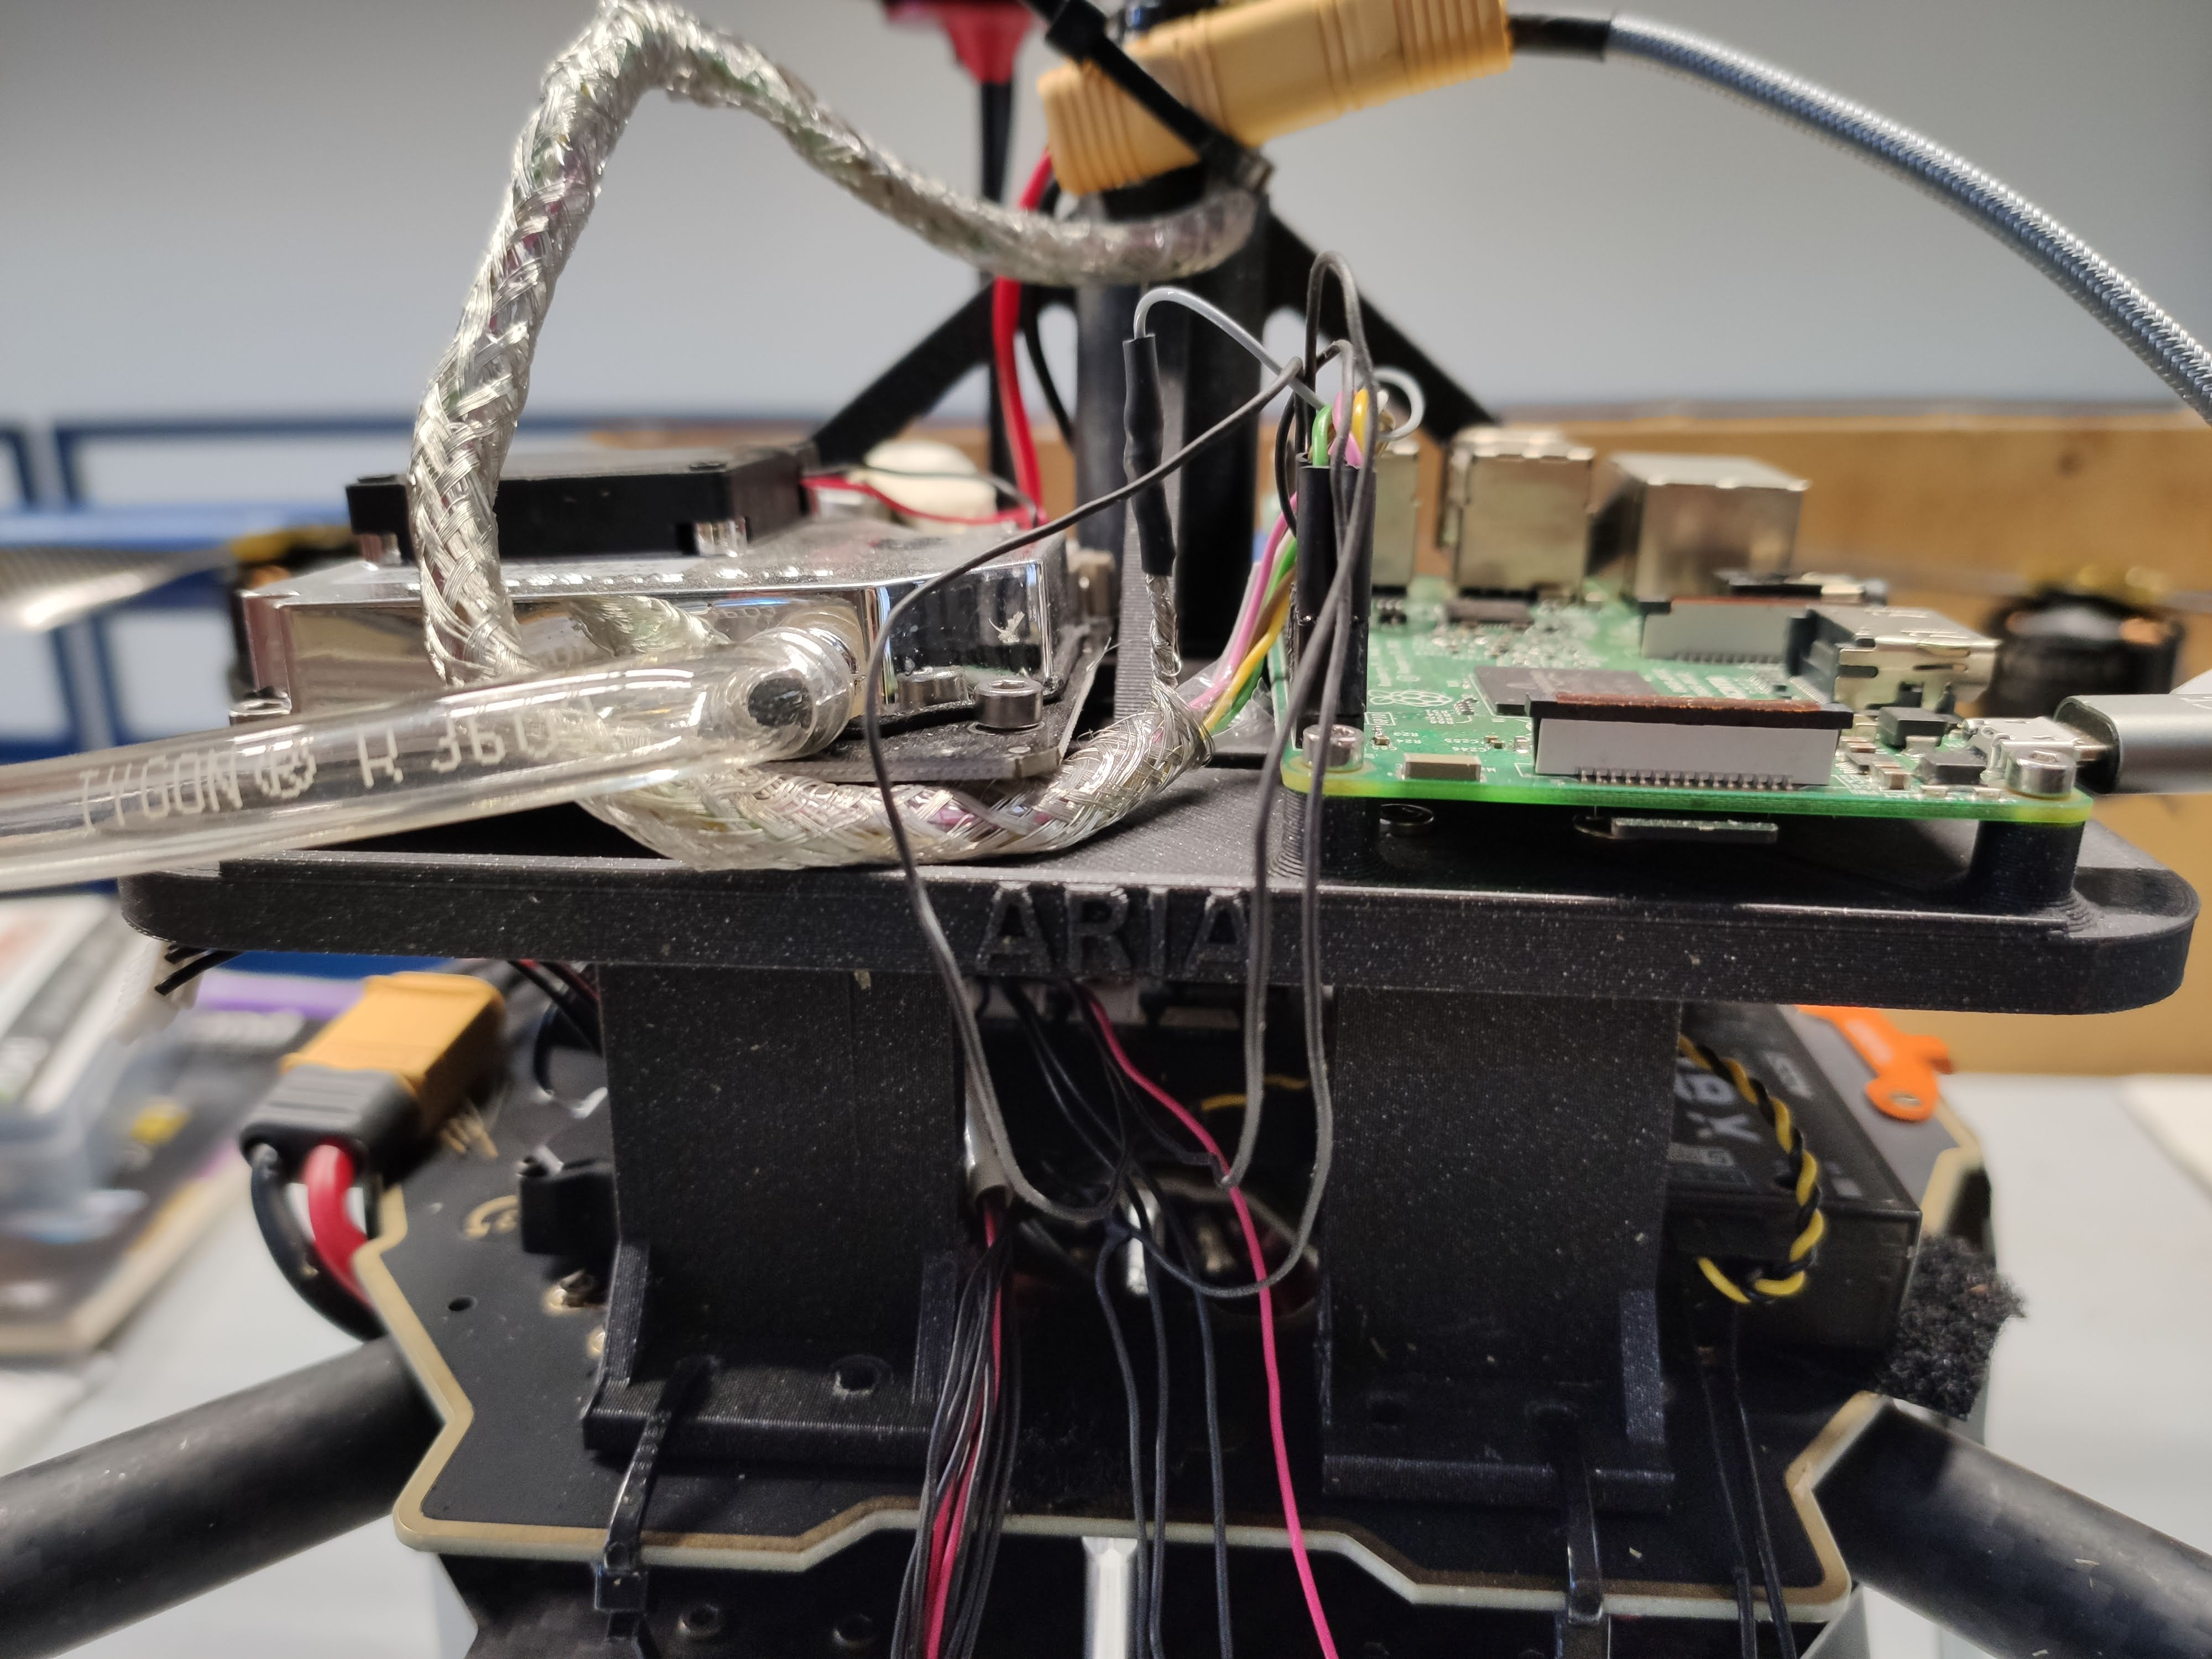
\includegraphics[width=\textwidth]{images/drone/IMG_20211105_103941.jpg}
        \caption{}
        \label{fig:pla1}
    \end{subfigure}
    \hfill
    \begin{subfigure}[b]{0.45\textwidth}
        \centering
        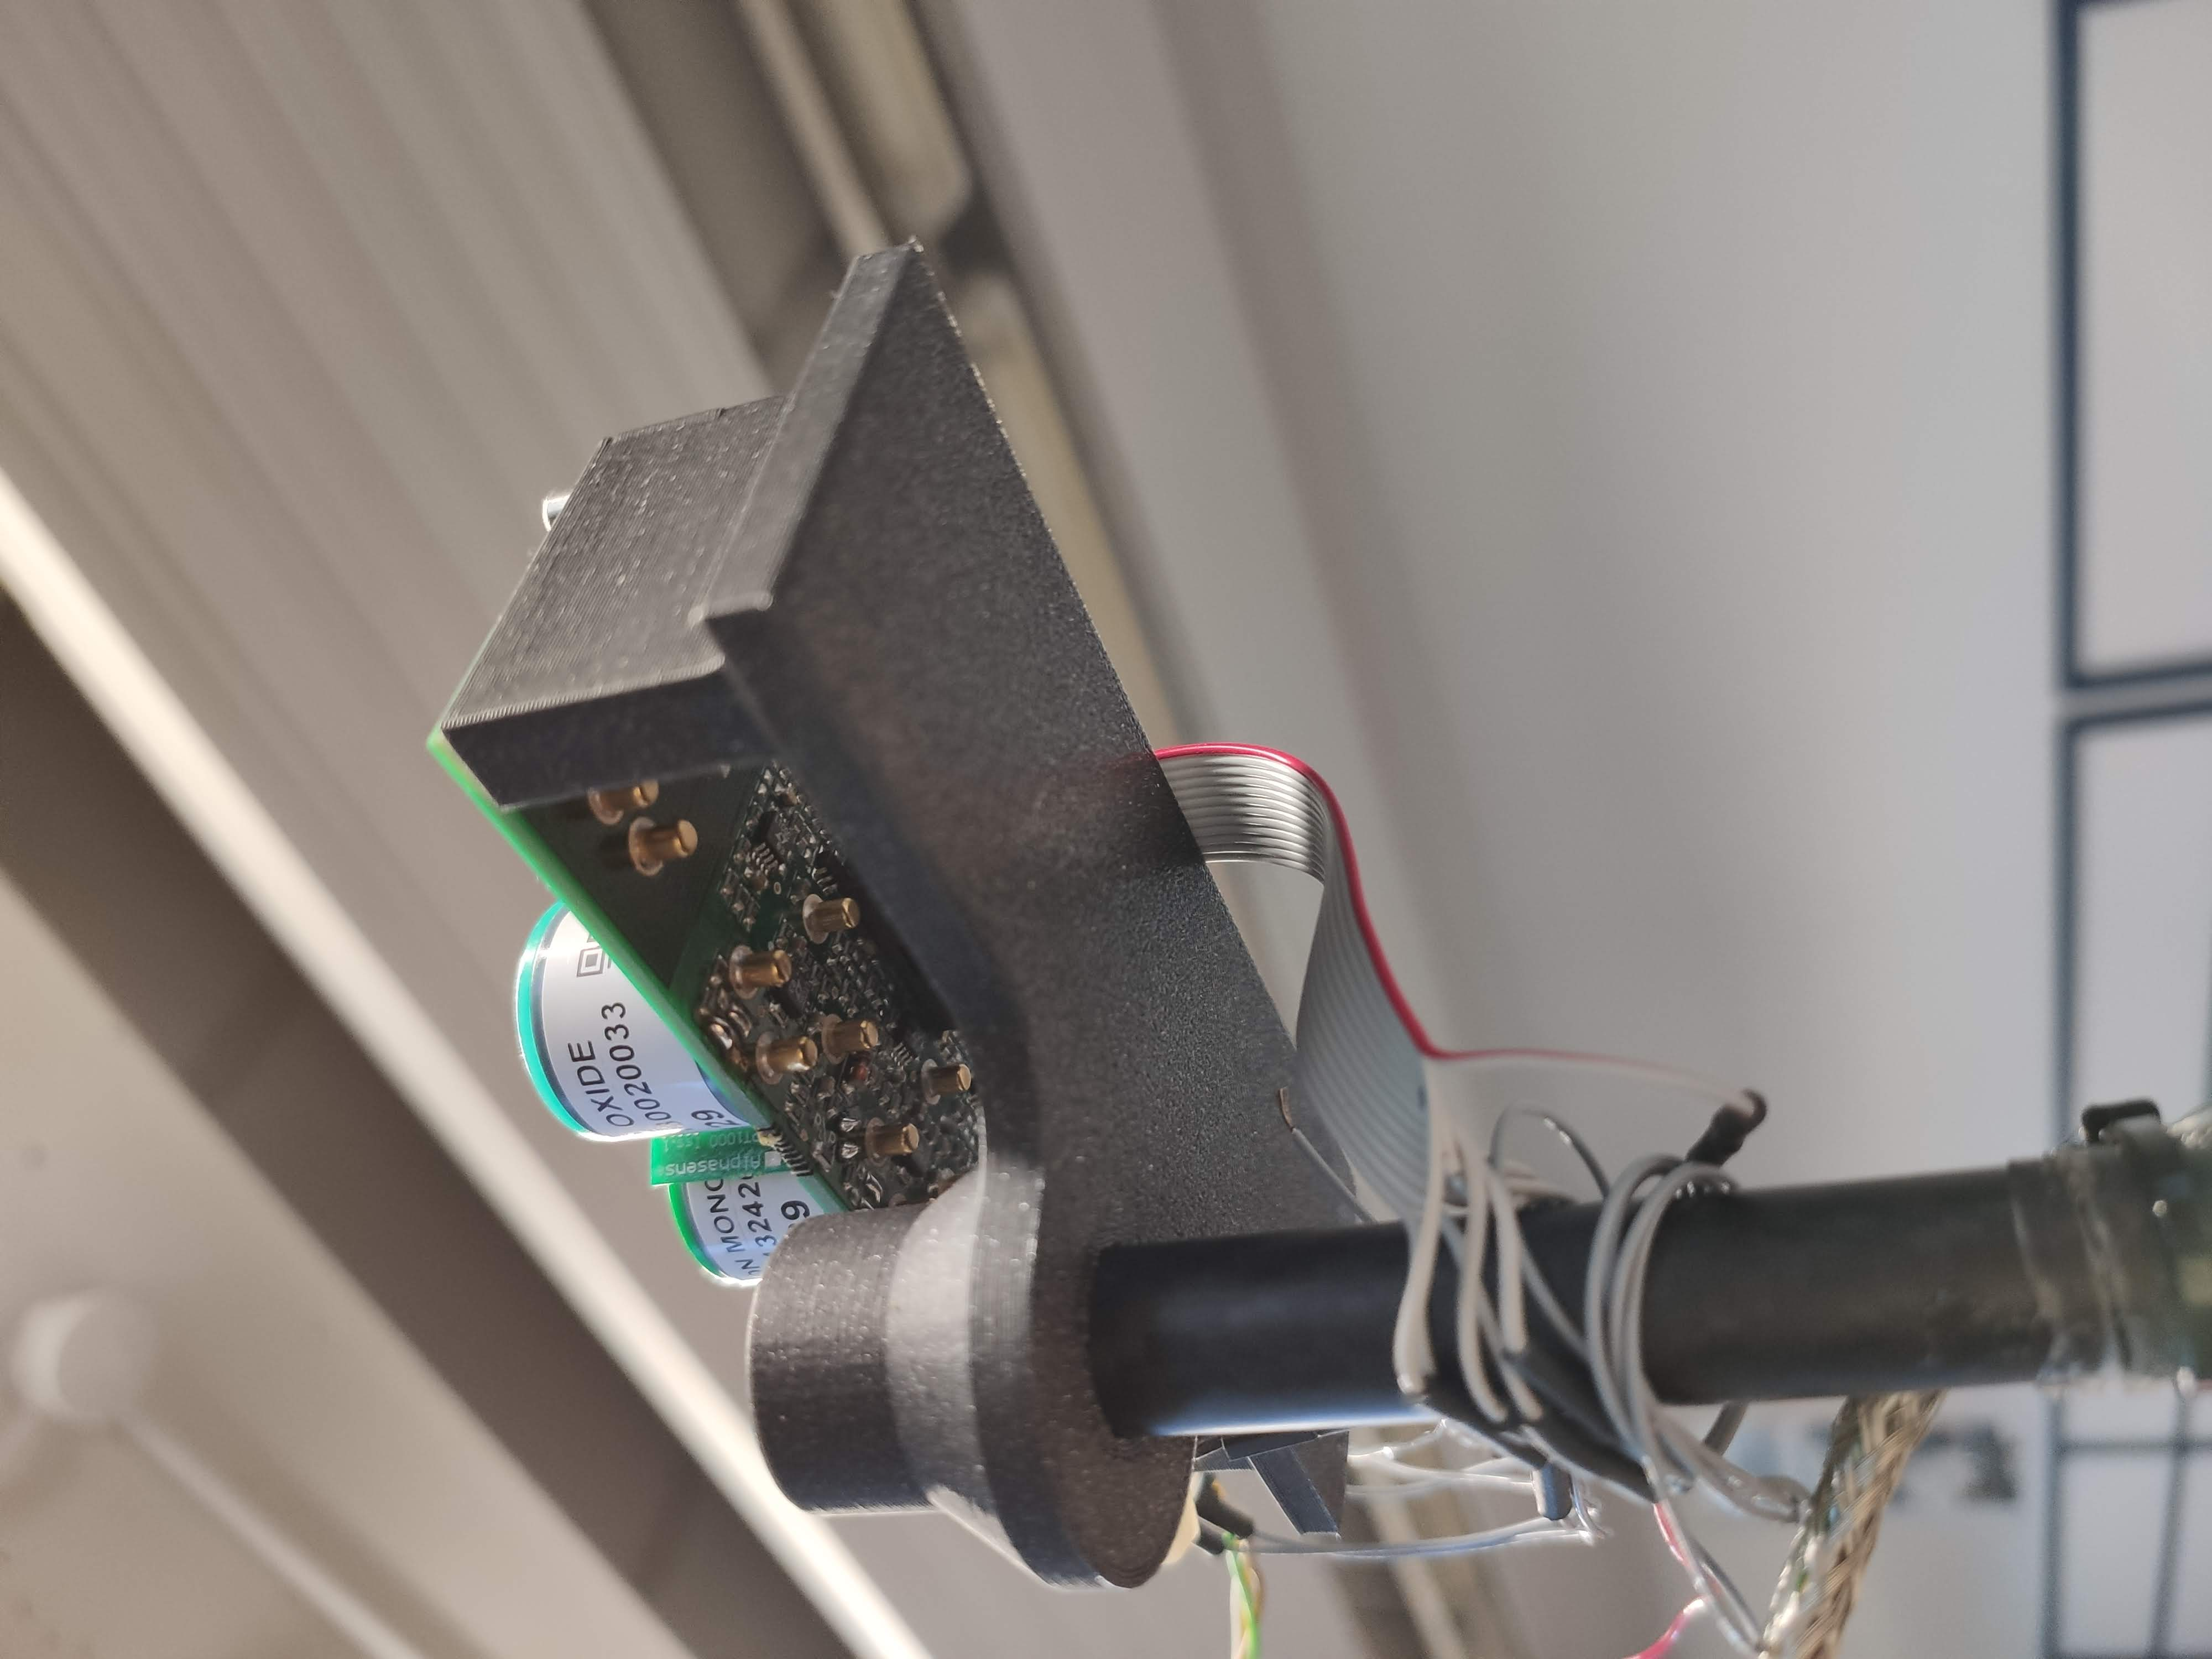
\includegraphics[width=\textwidth, angle=-90]{images/drone/IMG_20211105_115556.jpg}
        \caption{}
        \label{fig:pla2}
    \end{subfigure}
       \caption{The 3D printed boards}
       \label{fig:pla}
\end{figure}
\clearpage
\section{Particulate sensors}
The particulate sensor is a Nova SDS011 PM sensor able to measure PM2.5 and PM10
concentrations with a resolution of $0.3\mu g/m^3$; range of measurement is: $0 - 1 mg/m^3$ and the frequency
of output is 1 Hz. The sensor is a \gls{cots} sensor used for house and environmental monitoring with
consumption around 1 W. Tests on the sensor were performed in the lab and outputs were calibrated.
The sensor is equipped with a 10 cm inlet pipe (see Figure 2) in order to facilitate the inflow of the air
in the sensor. Sensor is linked to the Raspberry via a USB interface board allowing fast connection and
is located on the drone main platform.
\begin{figure}[h!]
    \centering
    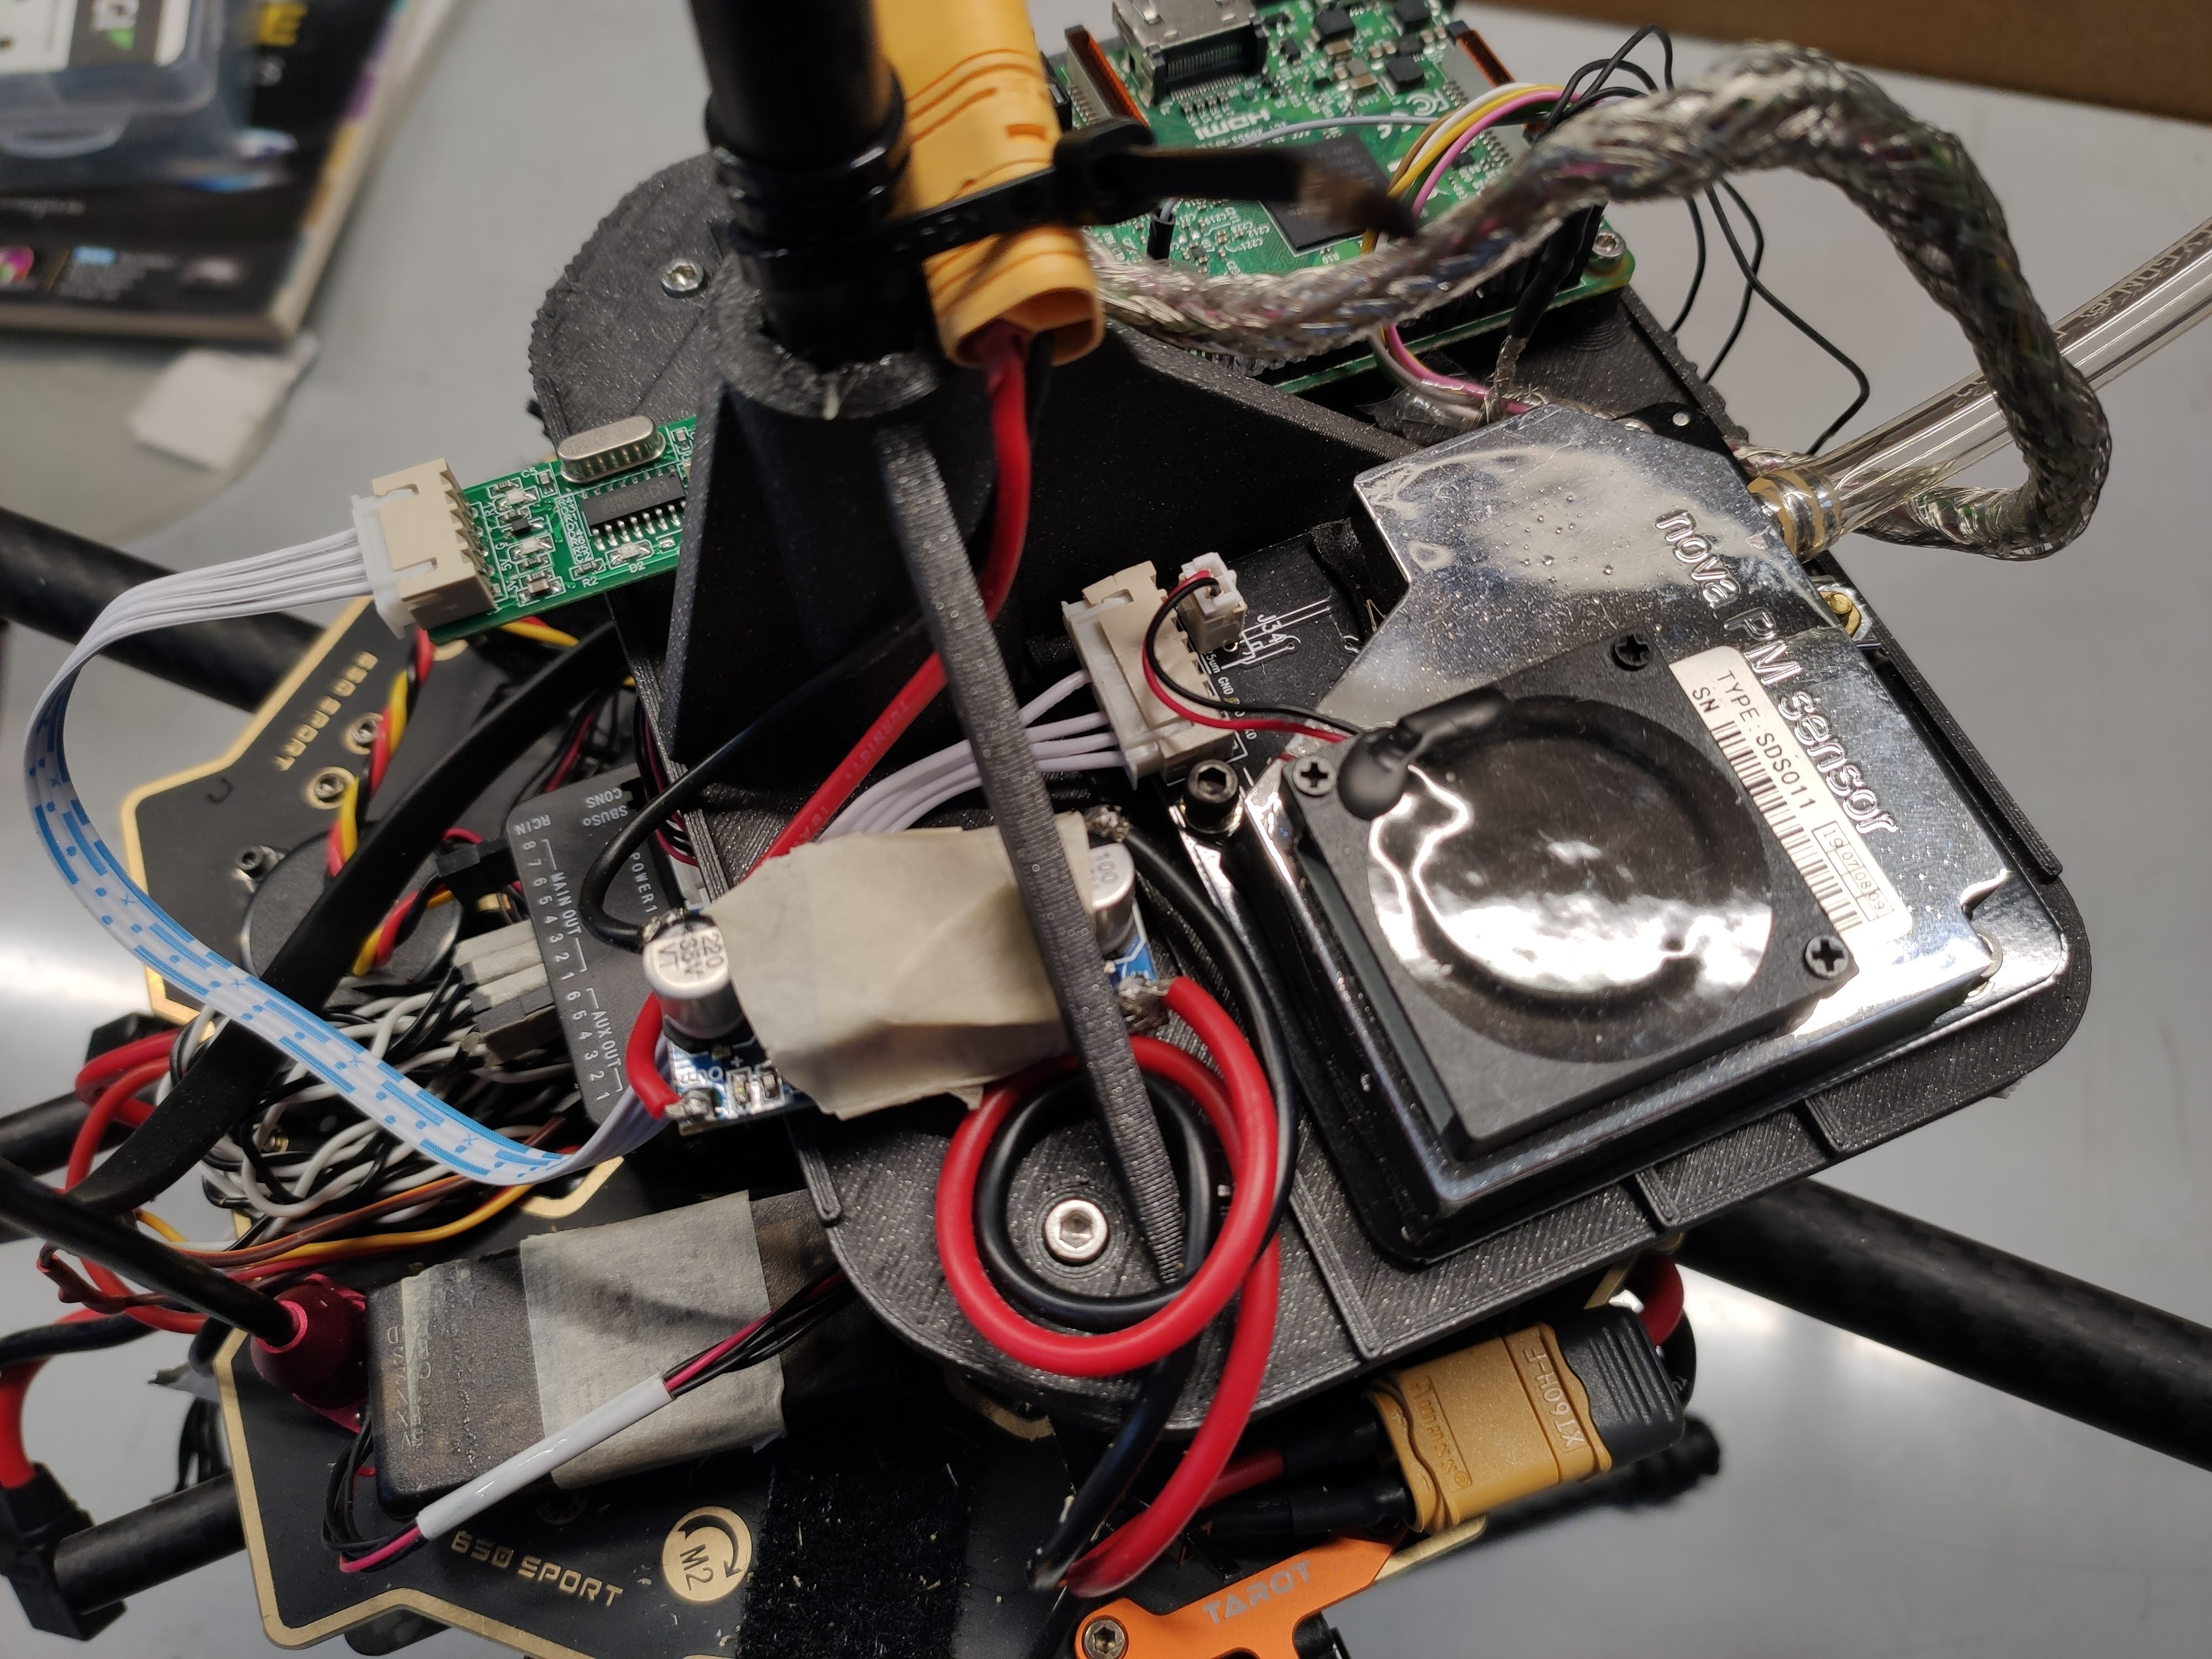
\includegraphics[width=0.7\textwidth]{images/drone/IMG_20211105_104126.jpg}
    \caption{The SDS011 particulate sensor and it's USB connected to the Raspberry Pi (partially covered by the pole structure)}
    \label{fig:sds011}
\end{figure}
\clearpage
\section{Gas sensors}
\begin{table}[H]
    \caption{\gls{aria}'s gas sensors}
    \centering
    \begin{tabular}{ |c|c|c|c|c| }
        \hline
        \thead{Substance} & \thead{Sensor} & \thead{Weight [g]} & \thead{Range [ppb]} & \thead{Data sheet} \\ [0.5ex]
        \hline
        \hline
        $CO$ & Alphasense CO-A4 & $< 6$ & 500 & \cite{co-a4} \\
        \hline
        $NO$ & Alphasense NO-A4 & $< 6$ & 20 & \cite{no-a4} \\
        \hline
        $NO_2$ & Alphasense NO-A43F & $< 6$ & 20 & \cite{no2-a43f} \\
        \hline
        $VOCs$ & Alphasense PID-AH2 & $< 8$ & \makecell{40 \\ (isobutylene)} & \cite{pid-ah2} \\
        \hline
    \end{tabular}
    \label{table:ariasensors}
\end{table}
They are connected to the Adafruit ADS1115 ADC and then to the raspberry. Due to 
The gas sensors have been positioned on a 50 cm boom in the center of the drone main platform
and above the drone itself (see Figure 2) in order to reduce disturbances due to variable flux moved
by the blades. Preliminary analysis show that the sensors are located in a non-altered flux allowing
for reliable measurements. Due to possible disturbances from electromagnetic sources present on the
drone (mainly telemetry antennas and electronics) a Faraday cage, not present in this study, but will be
built around the gas sensors and tested in future flights.
\begin{figure}[h!]
    \centering
    \begin{subfigure}[b]{0.45\textwidth}
        \centering
        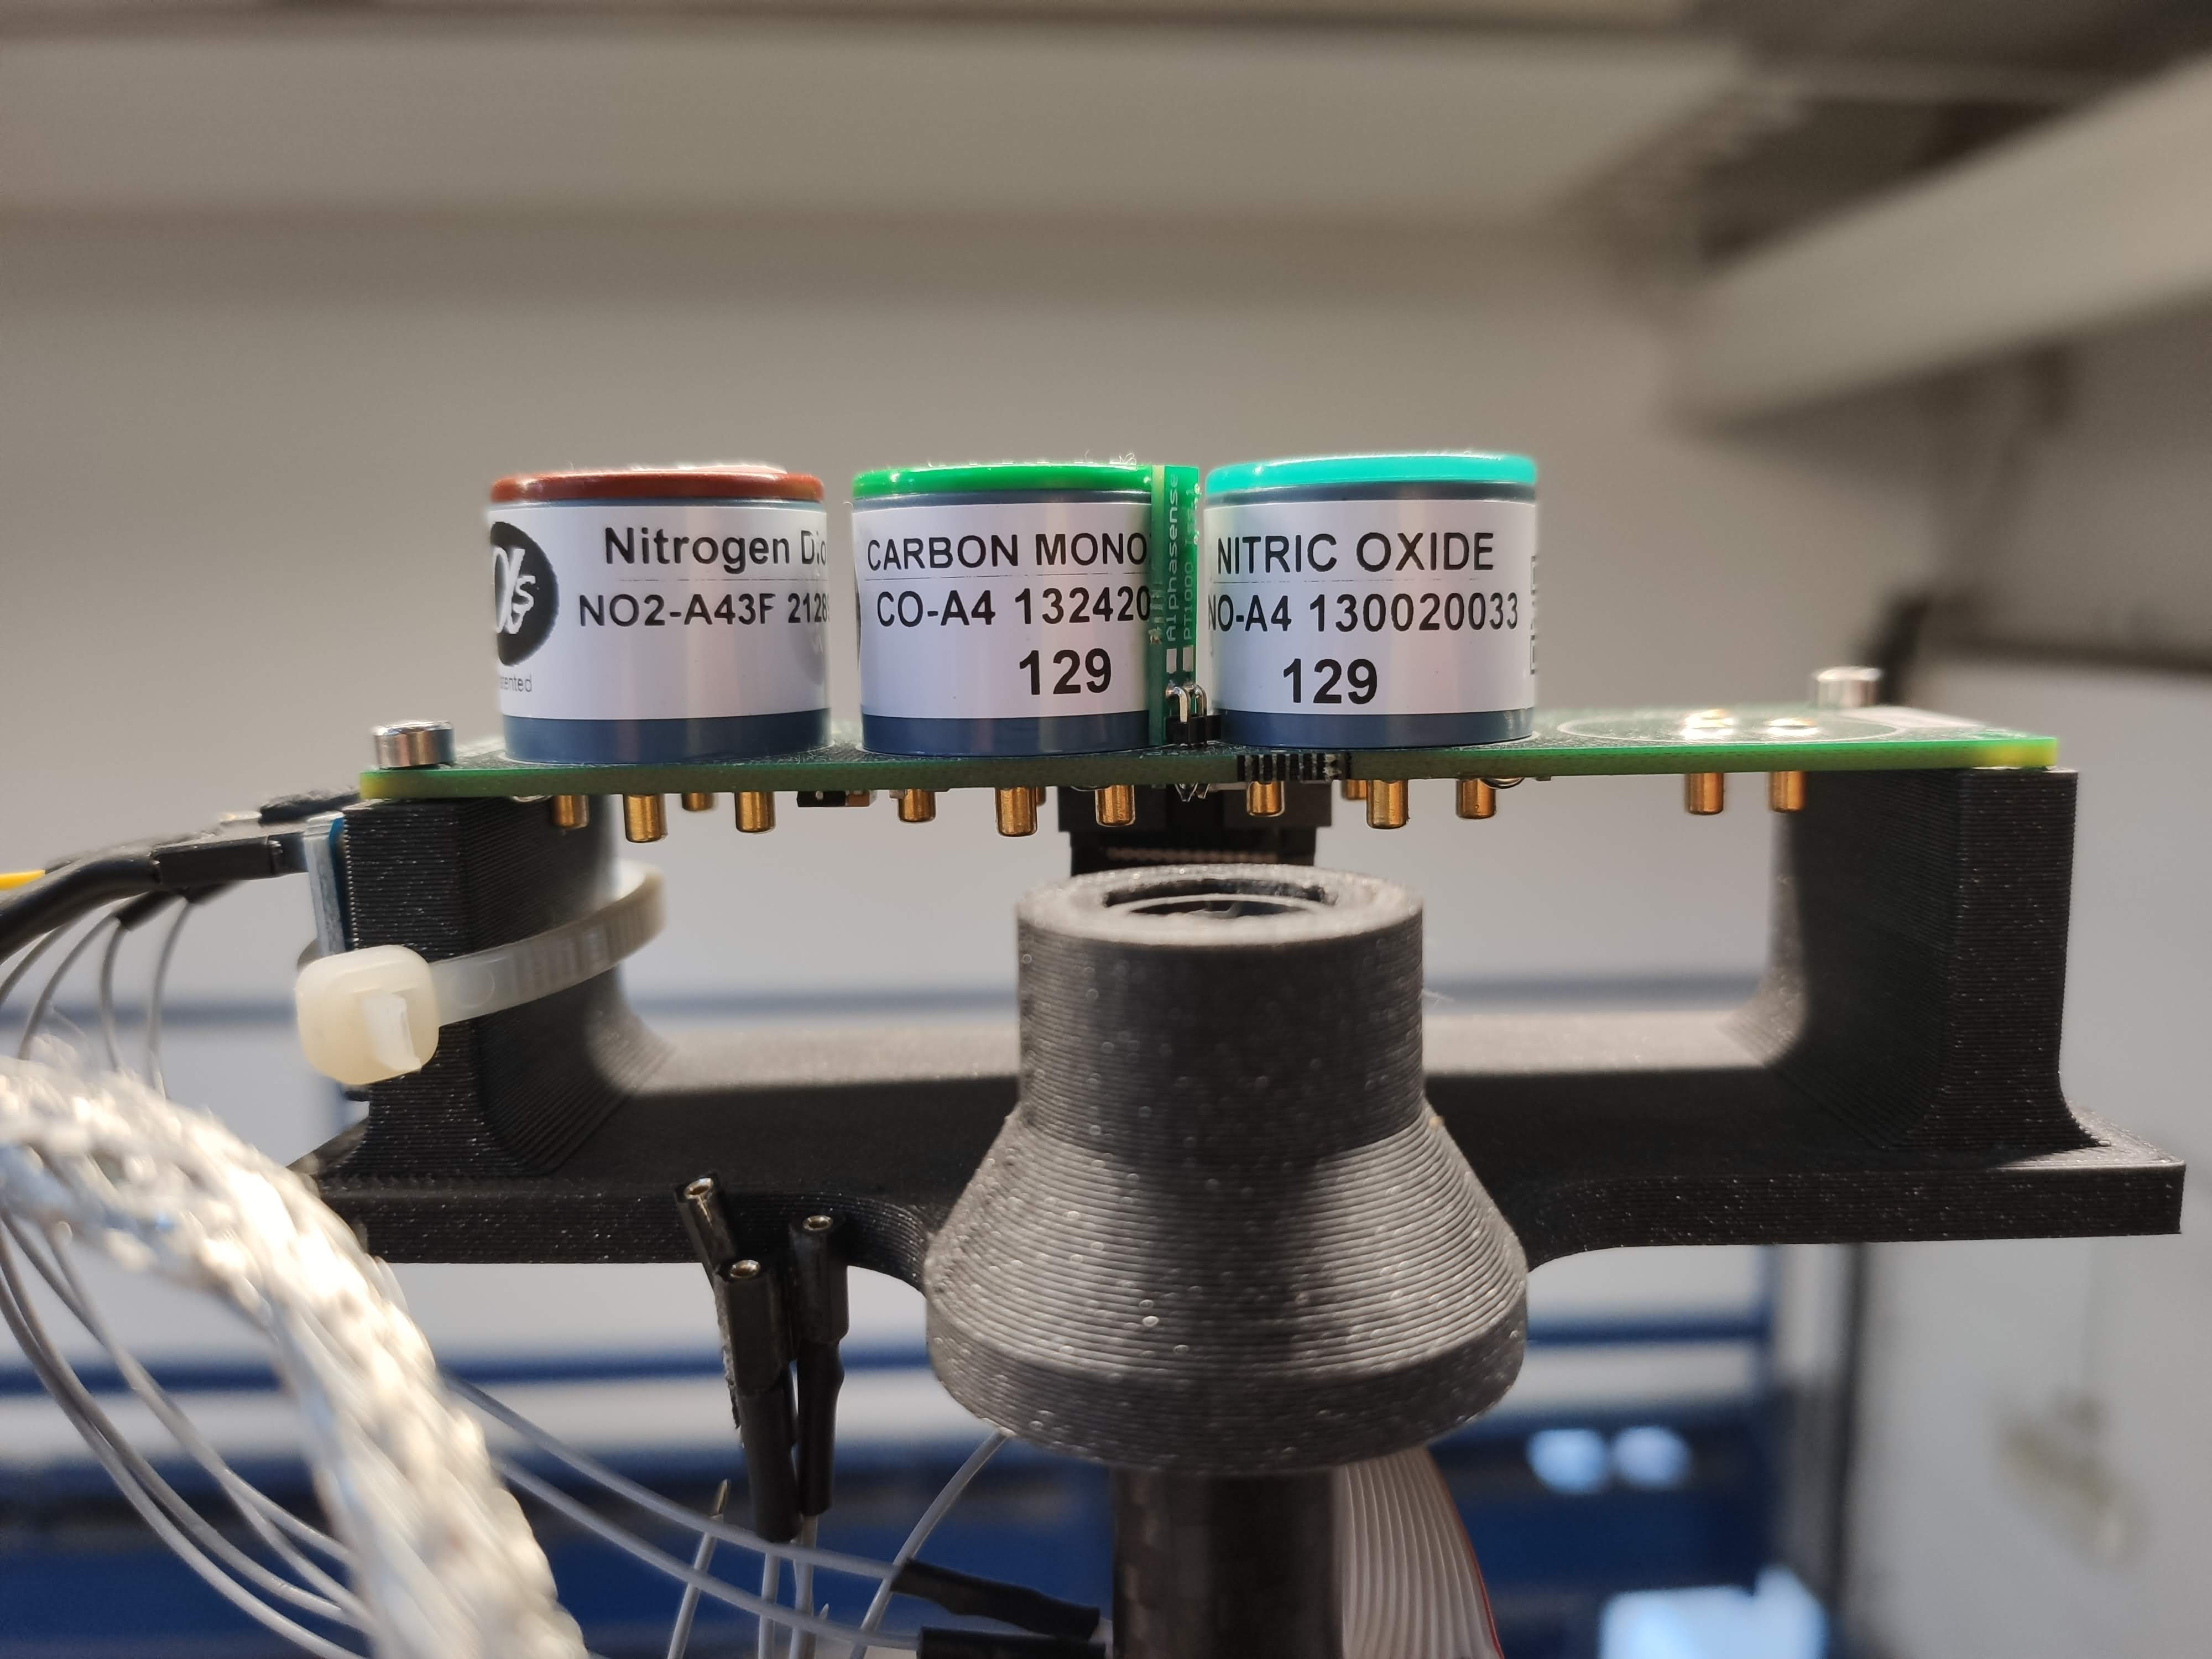
\includegraphics[width=\textwidth]{images/drone/IMG_20211105_104008.jpg}
        \caption{}
        \label{fig:gas-sensors1}
    \end{subfigure}
    \hfill
    \begin{subfigure}[b]{0.45\textwidth}
        \centering
        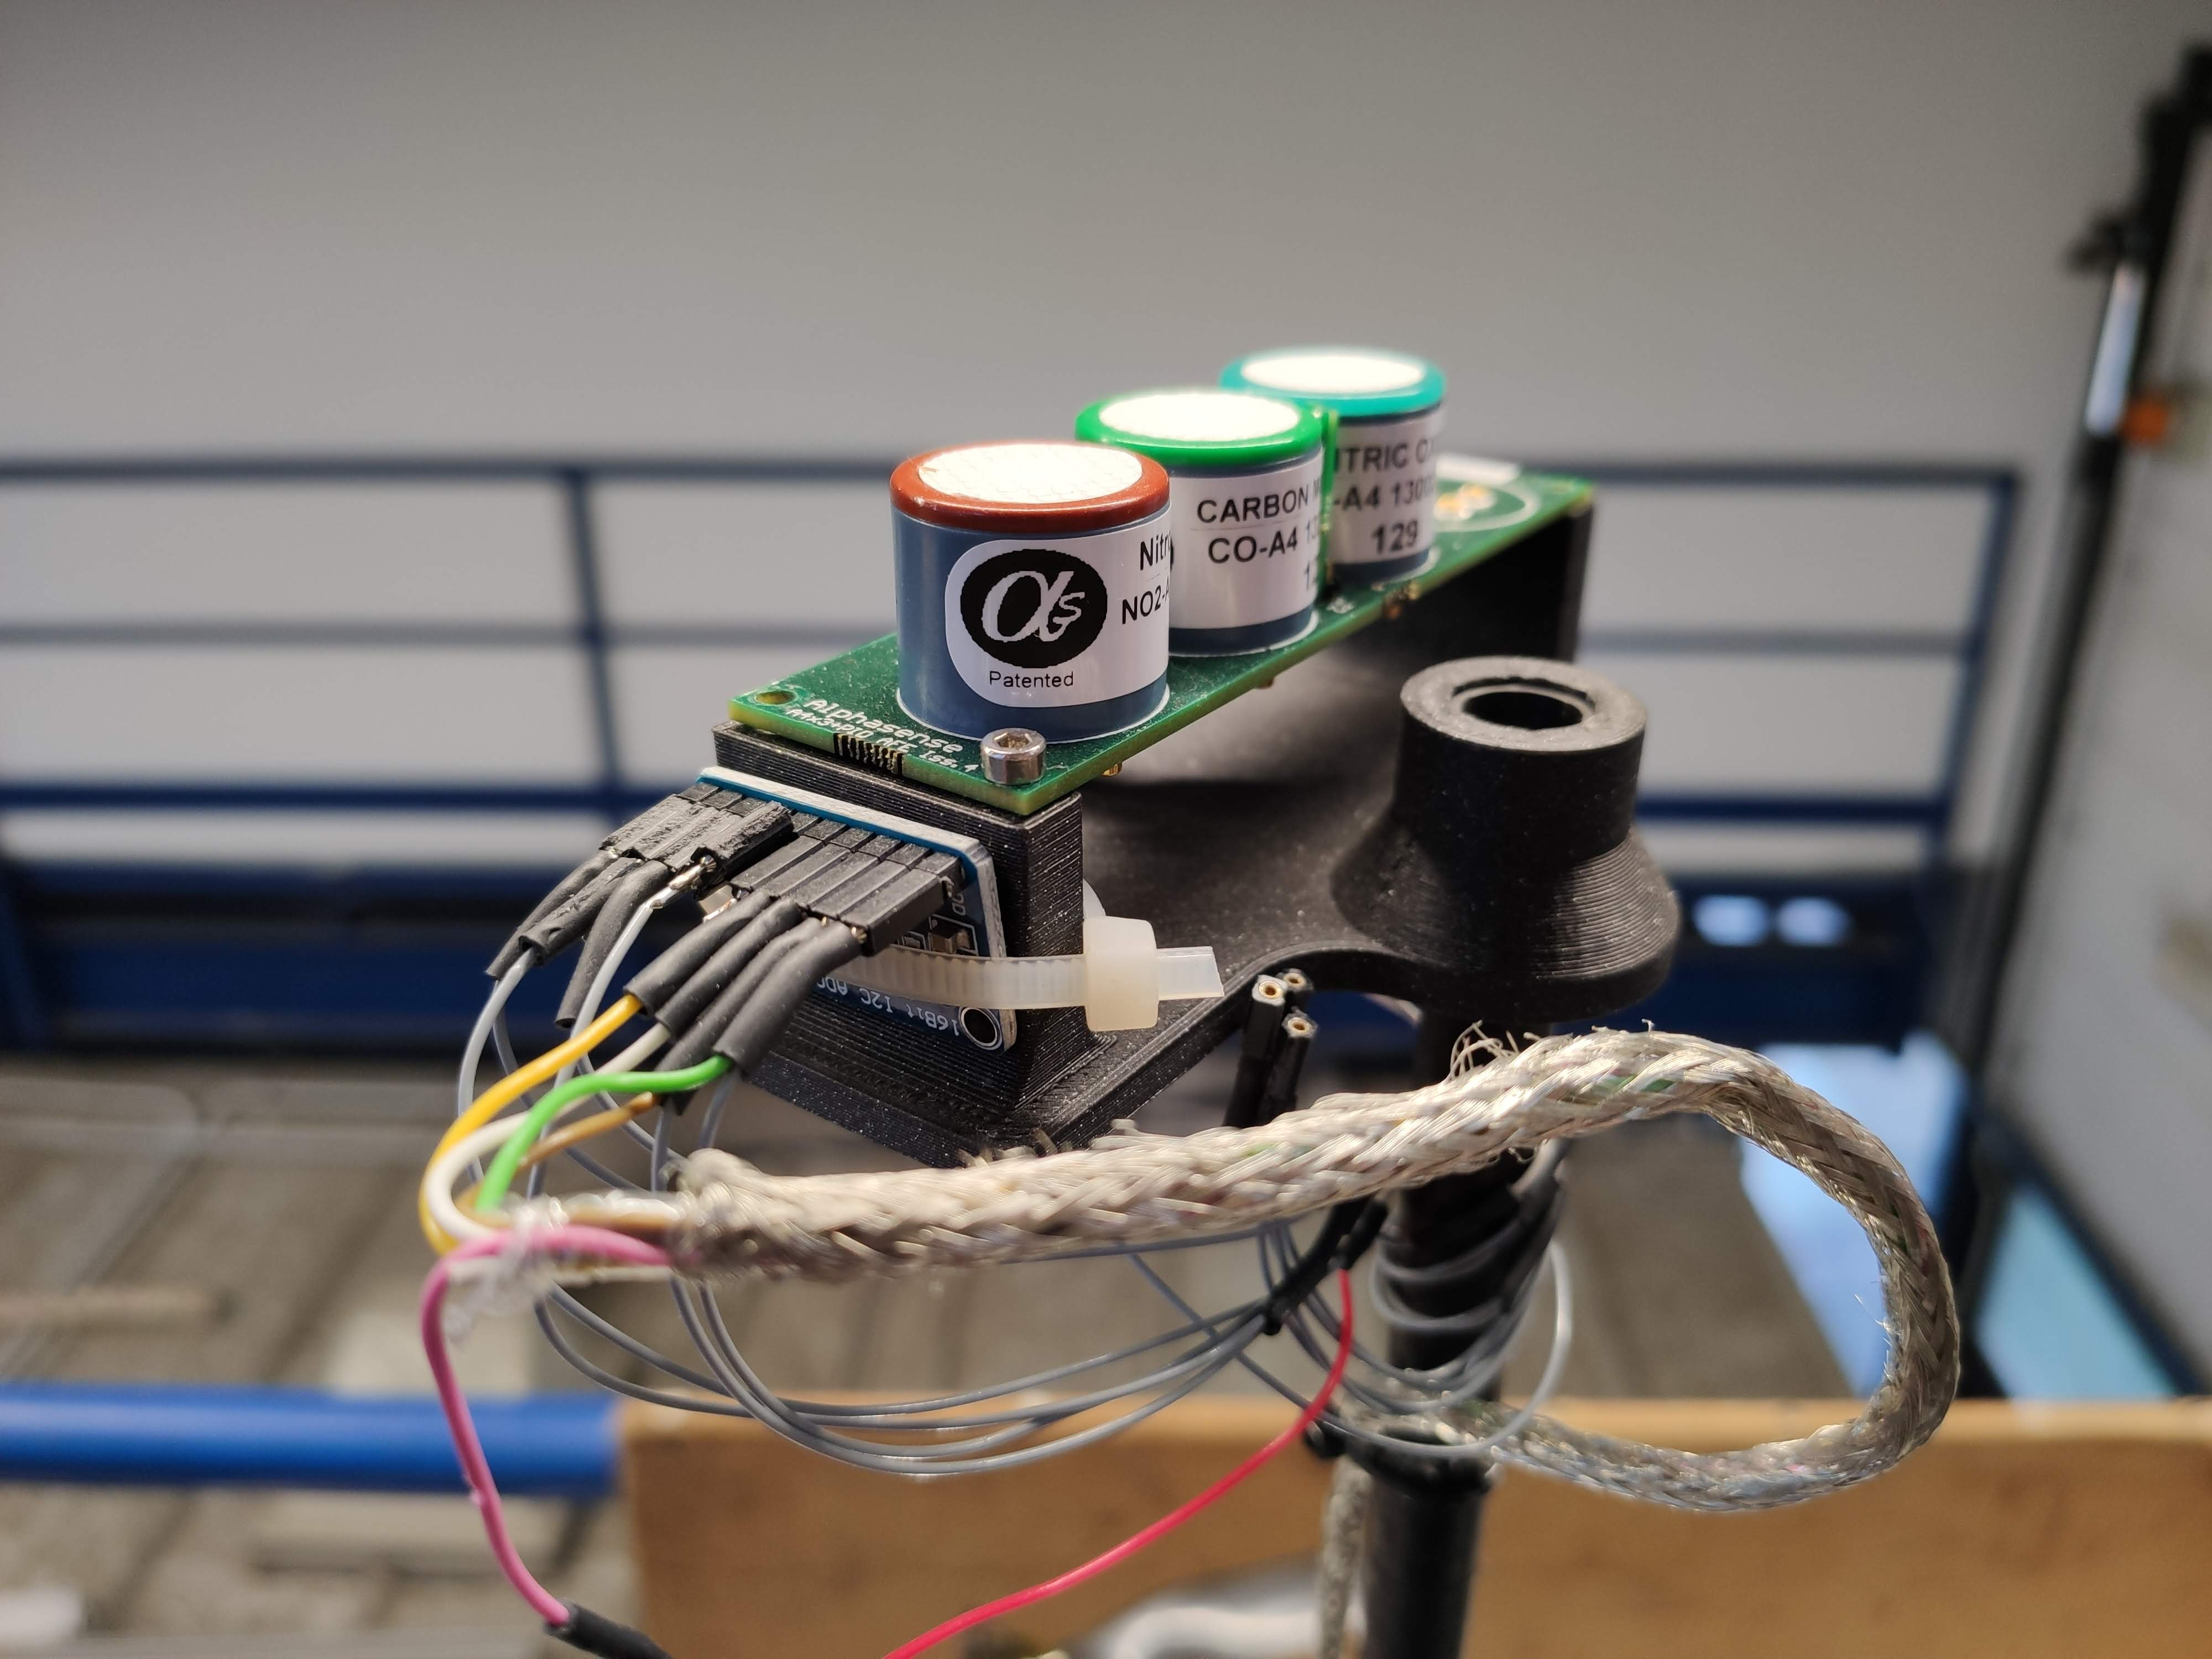
\includegraphics[width=\textwidth]{images/drone/IMG_20211105_104040.jpg}
        \caption{}
        \label{fig:gas-sensors2}
    \end{subfigure}
       \caption{The Alphasense gas sensors on the AFE board on top of the pole and the ADS1115 ADC on the side. The NO sensor is present but not connected.}
       \label{fig:gas-sensors}
\end{figure}
\clearpage


%sincronia con altro sistema arduino
%righe csv coerenti e synch
% picchi co semaforo, parco
%pm coincide, differenza data da pipetta
%fixare altitudine
%appendice formule